\section{Numerical Experiments}

In this section we run numerical experiments compairing the backward euler methods to Kyrlov methods for computing solutions to Allen Cahn equation with a traveling wave solution\cite{YukitakaFukao2004} given by:

\begin{align}
    \hat u(x,y,t)=\frac{e^{\frac{x-ct}{\sqrt2}}}{1+e^{\frac{x-ct}{\sqrt2}}} \label{TravelingWaveSol}
\end{align}
and where the problem is defined as follows:
\begin{align*}
    u_t&=\Delta u+u(u-\frac14)(1-u)\\
    \text{with } \Omega &= \mathbb{R}\times[-1,1]\\
    u(x,y,t) &= \hat u(x,y,t) \text{ for $(x,y,t) \in \mathbb{R}\times\{-1,1\}\times\mathbb{R}_+$}\\
    u_0 &= \hat u(x,y,0)\\
\end{align*}
However for our numerical experiments we compute on the space $\Omega=[-16,16]\times[-1,1]$.
We will use Neumann boundary on the left and right sides of the domain based on the exact solution given above and use a neumann boundary of $0$ along the top and bottom.
We give the PDE problem bellow and then write it in weak form.
\begin{align*}
    \dot u&=\Delta u+u(u-\frac14)(1-u)\\
    \int_{\Omega} \dot u v &=\int_{\Omega} \Delta uv+u(u-\frac14)(1-u)v\\
    \int_{\Omega} \dot u v &=\int_{\Omega} u(u-\frac14)(1-u)v - \nabla u \cdot \nabla v + \int_{\partial\Omega}  v\hat n \cdot \nabla u\\
    \text{subsituting in } u_h(t,x,y) &= \sum_i u_i(t) v_i(x,y)\\
    \text{we get } \int_{\Omega} \dot u_i v_i v_j &=\int_{\Omega} u_iv_i(u_iv_i-\frac14)(1-u_iv_i)v_j - \nabla (u_iv_i) \cdot \nabla v_j + \int_{\partial\Omega}  v_j\hat n \cdot \nabla \hat u_iv_i\\
    u_i\int_{\Omega}v_iv_j &= -u_i\int_{\Omega}\nabla v_i \cdot \nabla v_j + \int_{\Omega}R(u_h)v_j\\
    \text{where we have } R(u)&=u(u-\frac14)(1-u) + \int_{\partial\Omega}  \hat n \cdot \nabla \hat  u\\
    \intertext{writing in matrix form gives}
    M\dot u_h &= DN(u_h) + R(u_h)\\
\end{align*}

In the tests, we will investigate the relation between step size, $L_2$ error and call to the operator $N$ which will be a crude approximation to the computational cost.
We compare the Backward Euler, First and Second order expoenntial methods over grid sizes: $1024,$ $2048$ and with time step $\tau=8,4,2,1,0.5,0.25,0.125,0.0625,0.03125$.

\subsection{Results}

Bellow we show the $L_2$ error with respect to the time step $\tau$.

\begin{figure}[H]
    \centering
    \begin{minipage}{0.49\textwidth}
        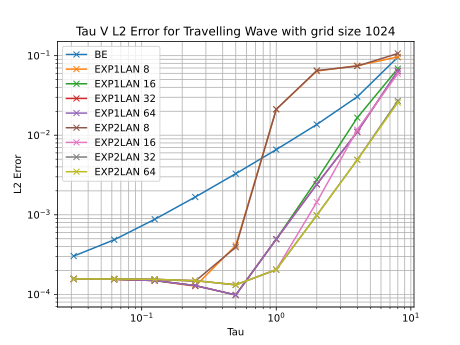
\includegraphics[width=1\textwidth]{Graphs/TravellingWave/Tau V L2 Error for Travelling Wave with grid size 1024.png} % Change filename to your image
        \caption{$\tau$ vs $L_2$ with grid size 1024}
        \label{fig:plot1}
    \end{minipage}\hfill
    \centering
    \begin{minipage}{0.49\textwidth}
        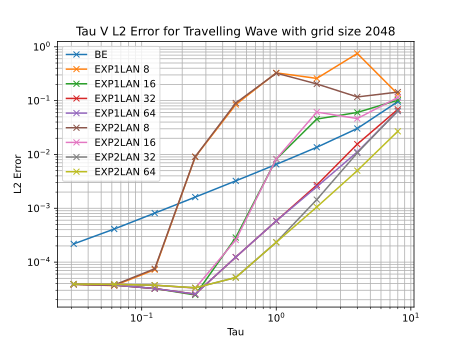
\includegraphics[width=1\textwidth]{Graphs/TravellingWave/Tau V L2 Error for Travelling Wave with grid size 2048.png} % Change filename to your image
        \caption{$\tau$ vs $L_2$ with grid size 2048}
        \label{fig:plot2}
    \end{minipage}\hfill
\end{figure}

We notice that when a smaller krylov subspace is used that the expoenntial methods only start to converge for a sufficiently small tau.
Likewise when these methods start to converge we observe that the perform simillarly to the methods using a larger subspace, however they will require fewer operator calls.
This suggests that for sufficient small time steps a shallower subspace may suffice.
Likewise for the converse that larger timesteps require a deeper krylov subspace.

Now we compare the error with the number of calls to the operator.
These operator calls are needed for computing $N$ which is used with the matrix free methods as described above as well as for computing the non-linear term $R$.

\begin{figure}[H]
    \centering
    \begin{minipage}{0.49\textwidth}
        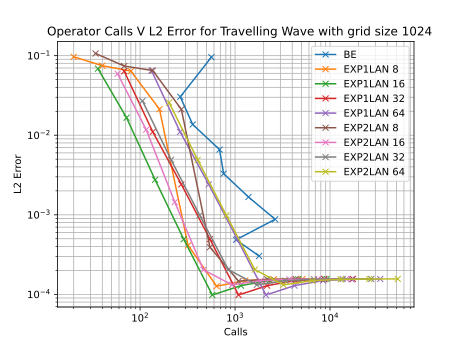
\includegraphics[width=1\textwidth]{Graphs/TravellingWave/Operator Calls V Error for Travelling Wave with grid size 1024.png} % Change filename to your image
        \caption{$\tau$ vs $L_2$ with grid size 1024}
        \label{fig:plot1}
    \end{minipage}\hfill
    \centering
    \begin{minipage}{0.49\textwidth}
        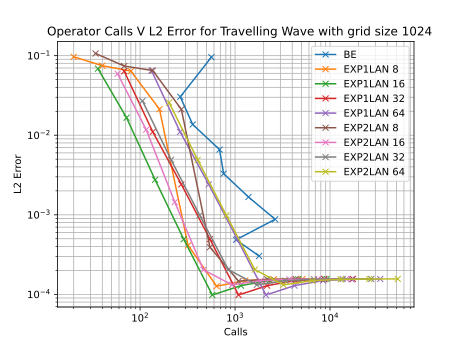
\includegraphics[width=1\textwidth]{Graphs/TravellingWave/Operator Calls V Error for Travelling Wave with grid size 1024.png} % Change filename to your image
        \caption{$\tau$ vs $L_2$ with grid size 2048}
        \label{fig:plot2}
    \end{minipage}\hfill
\end{figure}

We see that as expected that when are larger krylov subspace is used that more calls to the operator are required.
We also observe that the exponential methods outperform the BE by achieving a lower error with fewer calls to the operator.

Here we present the experimental orders of convergence.

\begin{table}[H]
    \centering
    \begin{tabular}{| c | c | c | c}
    \hline
    BE & EXP1LAN 64 & EXP2LAN 64 \\
    \hline
    1.656175178817219 & 2.5200121901844423 & 2.427488988868435 \\
    1.159963039219372 & 2.147211103525317 & 2.2448741639287576 \\
    1.0543798412512431 & 2.1084233436748687 & 2.175268892119002 \\
    1.0188791686457326 & 2.235535140373336 & 2.176237872787299 \\
    1.0016513655730614 & 2.2847781778148475 & 0.6355415381730404 \\
    0.9874831778164389 & -0.3463812590562603 & -0.1610890501147955 \\
    0.9808216274859436 & -0.2097197508087928 & -0.0545528584432596 \\
    0.919336864575657 & -0.051644372942987 & -0.01407844052927163 \\
    \hline
    \end{tabular}
    \caption{Reduced Data Table}
    \label{tab:reduced_data}
\end{table}

    


We observe that the rate of convergence for the second order method was inline with what has been shown analytic\cite{Huang2022} at a rate of $2$.
The first order method converges with a rate of 2 despite an expectation of a rate of $1$\cite{Huang2022}.
The backwards euler converges at the rate expceted of 1.